Die bearbeitete Aufgabe entspricht der zweiten der zur Verfügung stehenden Aufgaben: \textit{Zusammenhängende Komponenten}.

Zum Programmstart ist eine Matrix mit schwarzen und weißen Feldern gegeben (jedes Feld der Matrix kann als Pixel auf einem Bild aufgefasst werden). Ziel des Programms ist es, alle maximalen zusammenhängenden schwarzen Komponenten (eine Gruppe von schwarzen Feldern) zu finden. Eine Komponente gilt dann als zusammenhängend und maximal, wenn es in den umgebenden Feldern (direkt angrenzend) keine weiteren schwarzen Felder mehr gibt. Eine genaue Definition ist in der ausgegebenen Aufgabenstellung zu finden.

Ausgeben soll das Programm alle gefundenen maximalen schwarzen Komponenten, ihre Größe und eine exemplarische Koordinate in der Matrix (um sie beispielsweise lokalisieren zu können).

Ein Beispiel ist in Abb. \ref{fig:inputbsp} auf Seite \pageref{fig:inputbsp} zu sehen. In der angegebenen Matrix sind 4 maximale schwarze Komponenten mit den Größen 5, 5, 7 und 8. Exemplarische Koordinaten für die Komponenten sind $\{(0, 1), (5, 1), (1, 7), (1, 11)\}$ (beschrieben als Matrix-Indizes, nicht als kartesische Koordinaten).

\begin{figure}[tbhp]
	\centering
	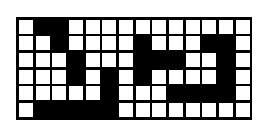
\includegraphics[width=0.7\textwidth]{images/inputbsp.eps}
	\caption{Beispielmatrix wie sie das Programm erwartet}
	\label{fig:inputbsp}
\end{figure}
